\section{Grundlagen}

In diesem Kapitel werden die zentralen Themen dieser Arbeit vorgestellt. Dazu
gehören die Funktionsweise von FreeRTOS, die Prinzipien von Caches sowie die
Erläuterung der \ac{DWT}.

\subsection{FreeRTOS}

FreeRTOS ist ein leichtgewichtiges, quelloffenes RTOS, das speziell für
Mikrocontroller und eingebettete Systeme entwickelt wurde. Es zeichnet sich
unter anderem durch ein echtzeitfähiges \cite{freertos_tutorial} und
deterministisches Ausführungsverhalten sowie eine Konfigurierbarkeit von
Heap-Allokationen aus.

FreeRTOS unterscheidet sich von der Bare-Metal-Programmierung dadurch, dass es
dem Nutzer einen umfangreichen Abstraktionslayer in Kombination mit einem
prioritätsbasierten Scheduling-Verfahren bereitstellt. Diese Abstraktionen
ermöglichen es, komplexe (Echtzeit-)Operationen zu bewältigen, ohne dass der
Nutzer die benötigten Funktionalitäten selbst implementieren muss. Beispiele
hierfür sind unter anderem Timer mit konfigurierbarer Genauigkeit (basierend auf
dem sogenannten Tick \cite{freertos_rtos_tick}), Queues, Semaphore sowie Mutexe.

Im Fokus dieser Arbeit stehen Queues für den Datenaustausch der
Steuerungssoftware sowie sogenannte „Direct Task Notifications“ zur
Inter-Task-Synchronisation. Ebenfalls relevant sind Mutexe und „Trace Hooks“ zur
Erfassung von Laufzeitdaten. Diese Komponenten werden im Folgenden detailliert
erläutert.

\paragraph{Queues}

Queues sind eine Kernkomponente von FreeRTOS. Sie ermöglichen nicht nur eine
Inter-Task-Kommunikation durch threadsicheren FIFO-Datenaustausch, sondern
dienen auch als Task-Synchronisationsmechanismen: Die Semaphore und Mutexe sind
schlicht auf Queues aufgebaut \cite{freertos_semphr_incl, freertos_queue_mtx}.

\paragraph{Semaphore und Mutexe} \label{sec:mutex}

Semaphore und Mutexe dienen zur der Koordination des Zugriffs auf gemeinsame
Ressourcen. Semaphore sind aber im Vergleich zu Mutexen besonders geeignet für
Inter-Task-Synchronisation aufgrund ihrer Einfachheit
\cite{freertos_semphr_doc}: Sie sind Synchronisationsmechanismen \textit{ohne}
Prioritätsvererbung -- ein Konzept, bei dem eine niedrig priorisierte Task, die
einen \textit{Mutex} hält, temporär auf die höhere Priorität der auf den Mutex
wartenden Task angehoben wird. Dieses Konzept ist kritisch für eine effiziente
Zugriffskoordinierung auf gemeinsame Ressourcen, was mit Semaphoren nicht
gewährleistet werden kann und folglich zu Prioritätsinversion führen kann: Eine
höher priorisierte Task wird blockiert, während der Scheduler eine andere,
niedriger priorisierte Task ausführt, die den geforderten Mutex möglicherweise
nicht besitzt -- und das so lange, bis die Task mit dem Mutex die Ressource
freigibt.

Die folgenden Sequenzdiagramme (\ref{fig:sequence_diagramm_invert},
\ref{fig:sequence_diagramm_inherit}) zeigen den Vergleich zwischen
Prioritätsinversion bei Verwendung eines Semaphors und der Prioritätsvererbung
bei einem Mutex, dargestellt an drei Tasks mit unterschiedlichen
Prioritätsstufen.

\begin{figure}[H]
    \centering
    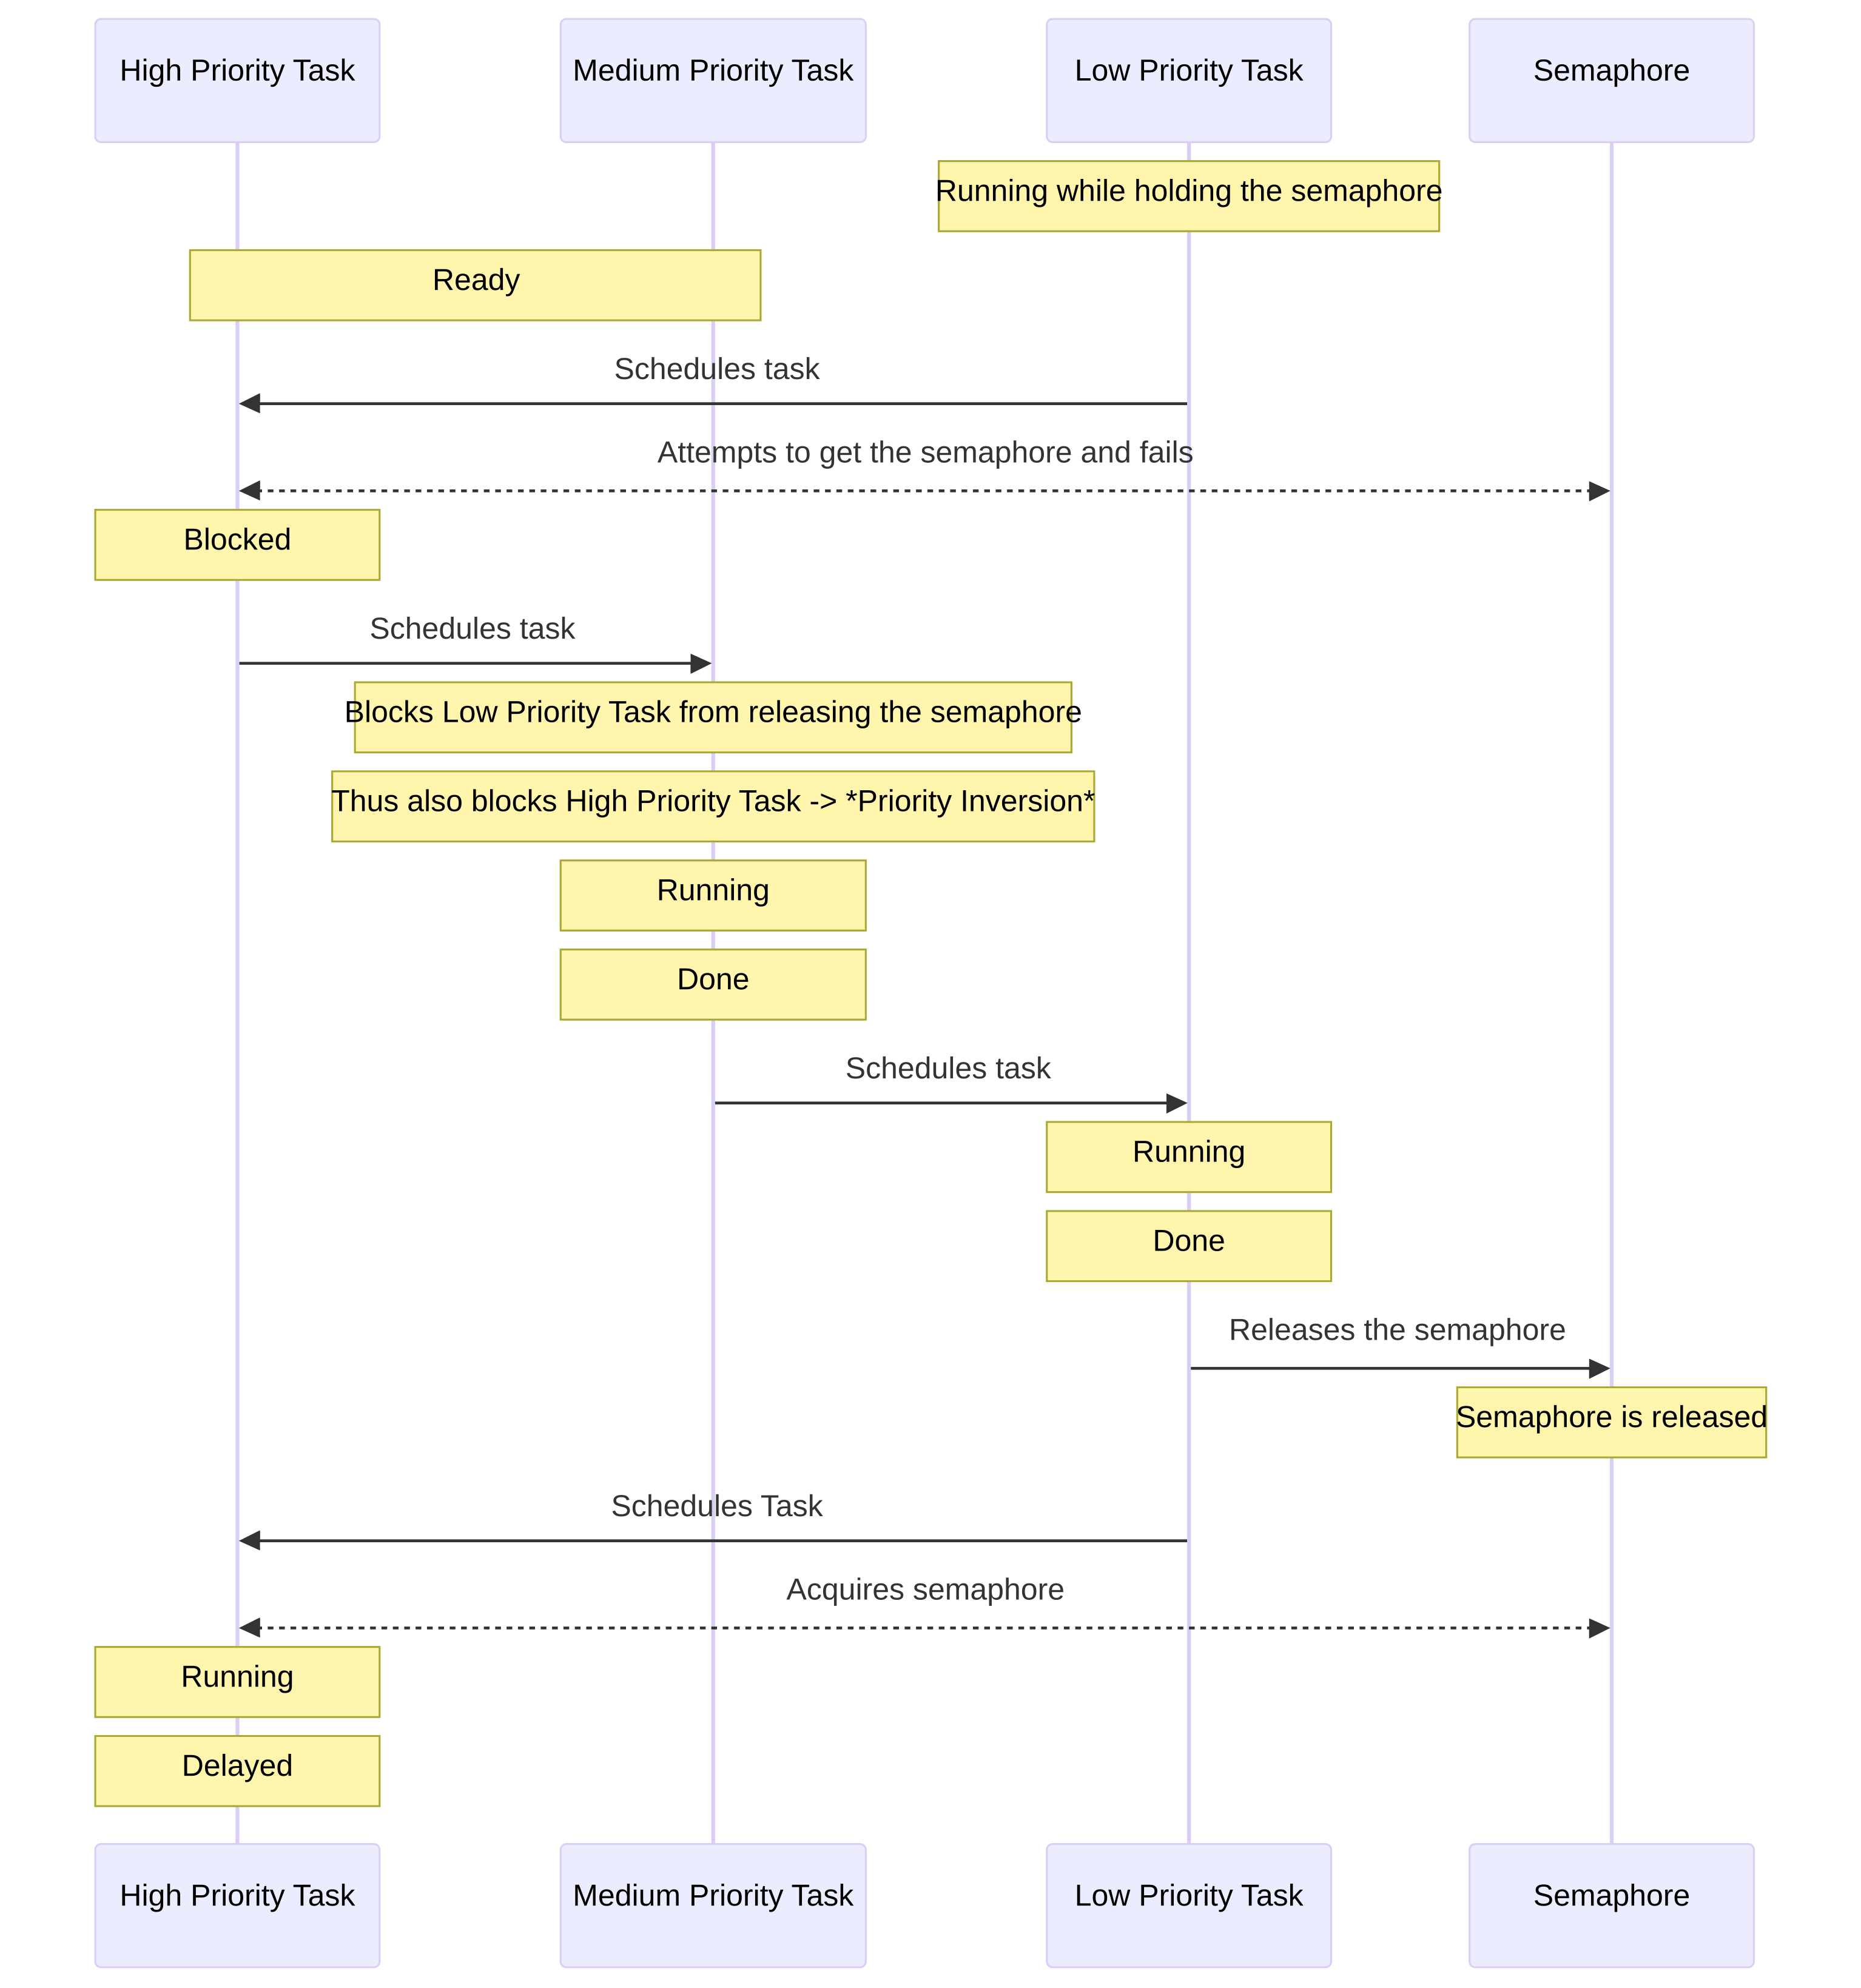
\includegraphics[width=1\textwidth]{assets/prio_inversion}
    \caption{Prioritätsinversion}
    \label{fig:sequence_diagramm_invert}
\end{figure}

\begin{figure}[H]
    \centering
    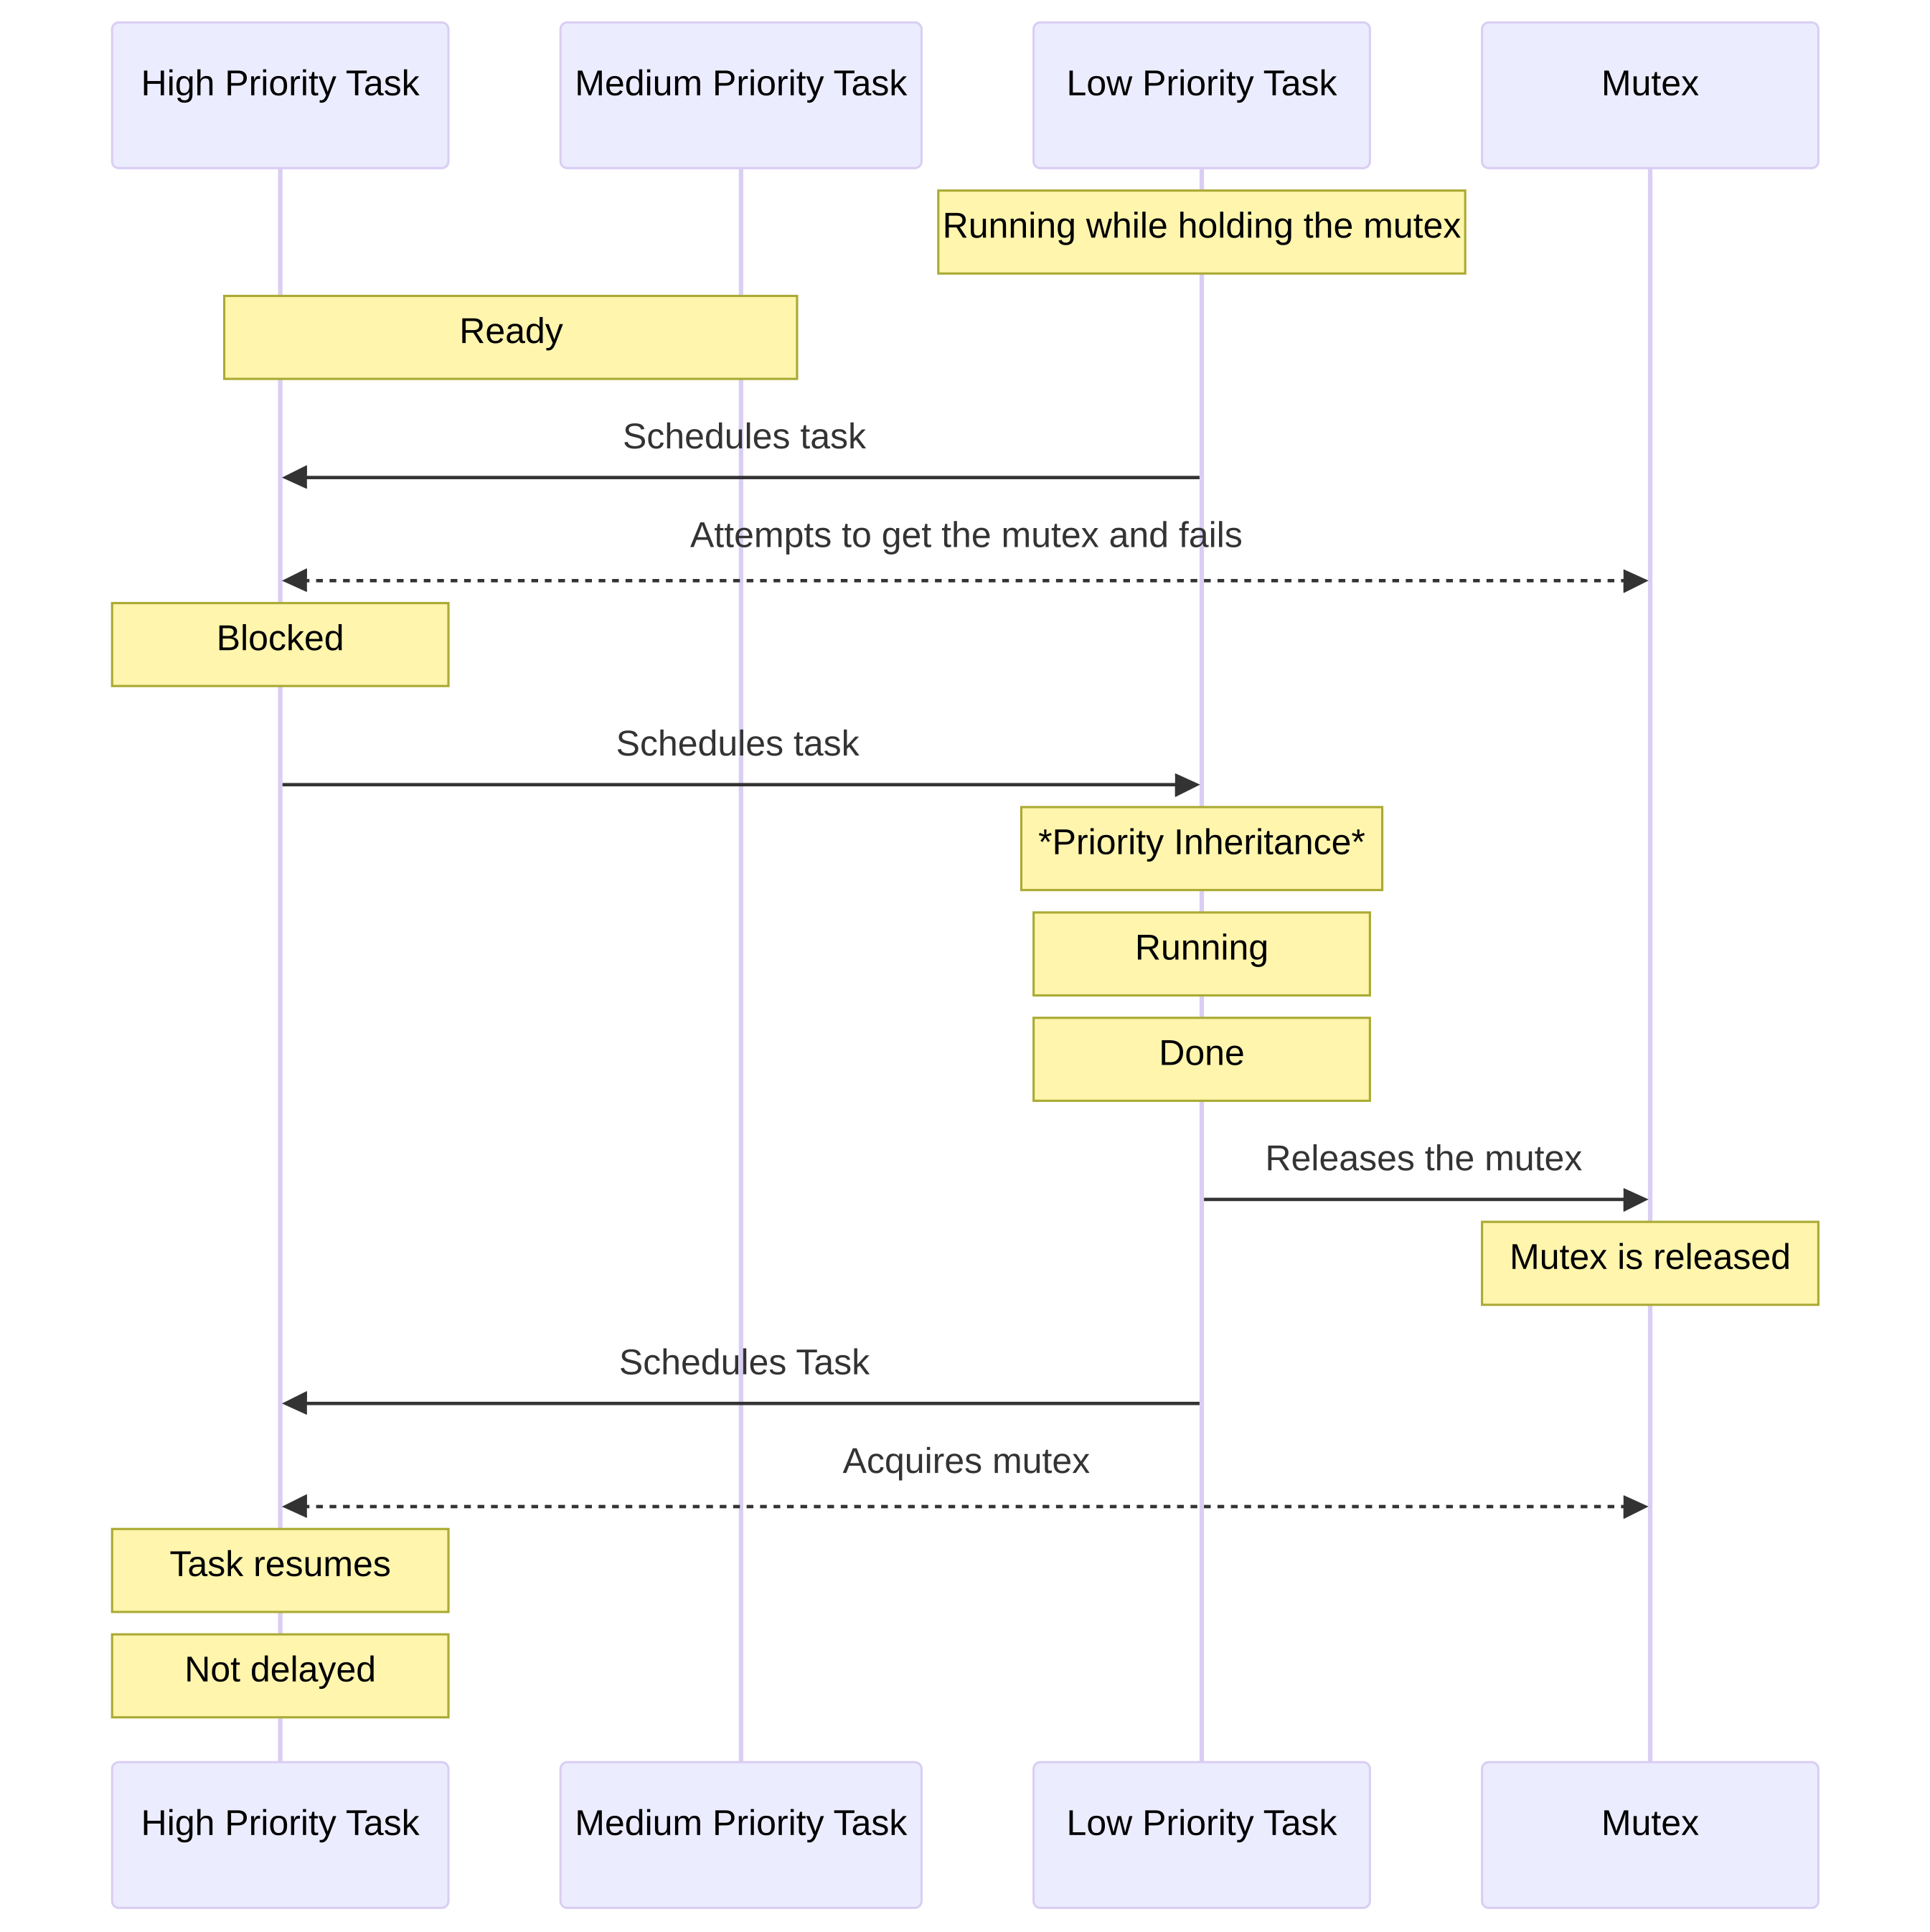
\includegraphics[width=1\textwidth]{assets/prio_inheritance}
    \caption{Prioritätsvererbung}
    \label{fig:sequence_diagramm_inherit}
\end{figure}

\paragraph{Direct-Task-Notifications} \label{sec:direct_task_notification}

Direct-Task-Notifications sind ein effizienterer und ressourcenschonenderer
Mechanismus zur Inter-Task-Synchronisation: Insbesondere soll das Entblocken
mittels Direct-Task-Notifications bis zu $45\,\%$ schneller sein und weniger RAM
benötigen \cite{freertos_task_notifications_usage}. Im Gegensatz zu Semaphoren,
die als zusätzliche separate Objekte fungieren, koordinieren die Tasks direkt
miteinander über einen internen Zähler \cite{freertos_tasks_c_308}. Analog zur
Verwendung von Semaphoren wird mittels Funktionen wie
\mintinline{c}|xTaskNotifyGive()| dieser Zähler
inkrementiert~\cite{freertos_tasks_c_4990}, während
\mintinline{c}|ulTaskNotifyTake()| ihn wieder
dekrementiert~\cite{freertos_tasks_c_4614}.

\paragraph{Trace Hooks} \label{sec:trace_hooks}

„Trace Hooks“ sind spezielle, von FreeRTOS bereitgestellte Makros. Sie
ermöglichen beispielsweise die Verfolgung bzw. Protokollierung von
Systemereignissen. Diese Makros werden direkt innerhalb von Interrupts beim
Scheduling aufgerufen und sollten stets vor der Einbindung von
\mintinline{text}|FreeRTOS.h| definiert werden \cite{freertos_rtos_trace_hooks}.

\subsection{Caches}

Caches sind schnelle Speicherkomponenten, die häufige Daten- und Befehlzugriffe
beschleunigen und den Energieverbrauch senken, wodurch jedoch die
Determinierbarkeit der Leistung verringert wird \cite{ka001150}. In modernen
Mikrocontrollern wie dem Cortex-M7 ist der L1-Cache (Level 1 Cache -- die
kleinste aber schnellste Cachekomponente) jeweils in einen Datencache (D-Cache)
sowie einen Instruktionscache (I-Cache) unterteilt \cite[S. 6]{an4667}. Im
Vergleich zum Flash-Speicher, bei dem Zugriffe mehrere Taktzyklen
erfordern~\cite{stm32_memory_sections}, ermöglichen L1-Caches
Zero-Wait-State-Zugriffe~\cite[S. 6]{an4667}. Dadurch kann der Prozessor ohne
zusätzliche Wartezyklen auf Daten zugreifen.

Der L1-Cache kann nur mit der \ac{AXI}-Busschnittstelle genutzt werden~\cite[S.
4]{an4839}. Hierzu zählen unter anderem der Flash, der \ac{SRAM} sowie die
Peripheriebusse, die alle über den \ac{AHB} an die AXI angebunden sind
(\ref{fig:m7_sys_arch}).

\begin{figure}[htb]
    \centering
    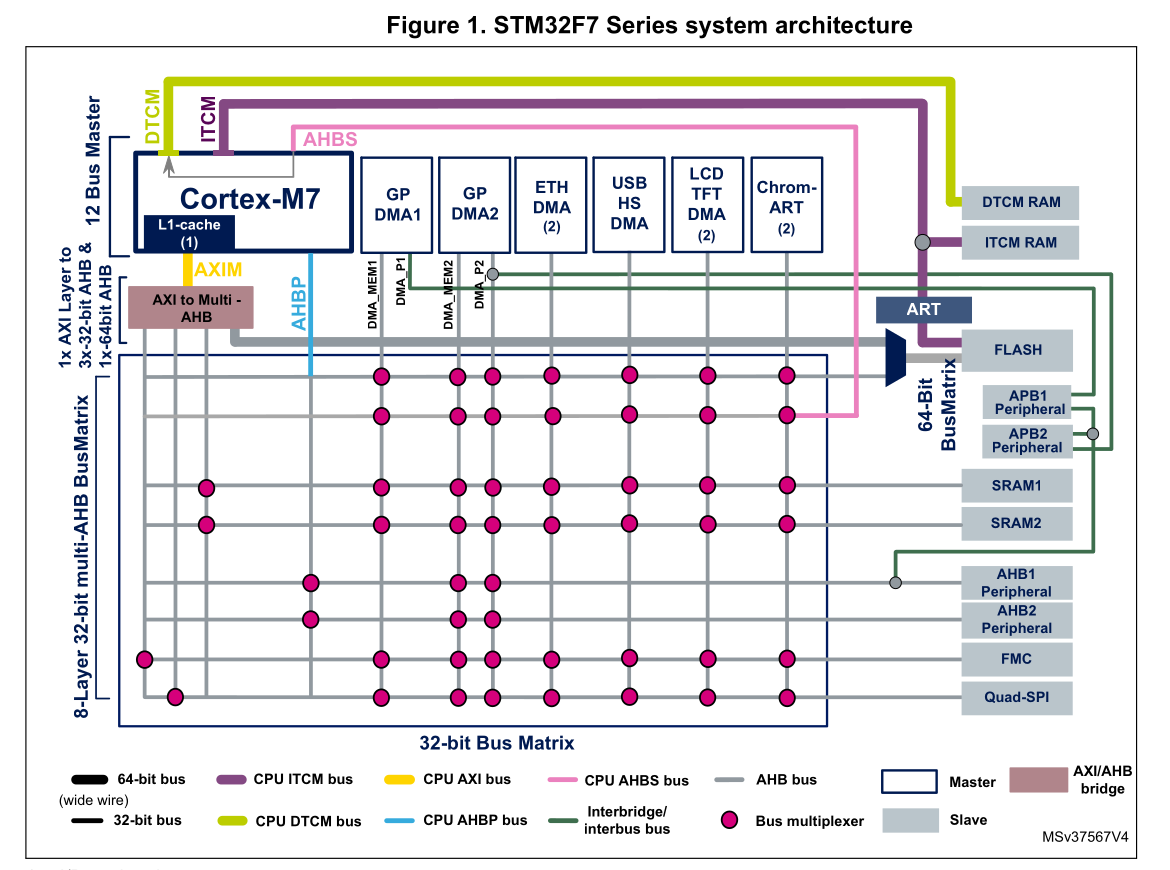
\includegraphics[width=1\textwidth]{assets/m7_system_arch}
    \caption{STM32F7 Systemarchitektur-Matrix \cite[S. 9]{an4667}}
    \label{fig:m7_sys_arch}
\end{figure}

Aus der Matrix wird außerdem deutlich, dass für den Speicher zwischen SRAM und
\ac{TCM}-RAM unterschieden wird. Der TCM verfügt jeweils für Instruktionen und
Daten über einen dedizierten Kanal direkt zum Prozessor und ist \textit{nicht}
cachefähig, bietet aber als Besonderheit niedrigere und konsistentere
Zugriffszeiten als SRAM. Dies macht es besonders geeignet für zeitkritische
Routinen, wie beispielsweise Interrupt-Handler. (\cite{arm_den0042})

Im Rahmen dieser Bachelorarbeit wird der TCM nicht genutzt und daher nicht
weiter betrachtet.

Zusammenfassend lässt sich sagen, dass jeder normale Speicherbereich (kein
Shared-Memory, Device-Memory oder Strongly-Ordered-Memory) gecacht werden kann
\cite[S. 7]{an4667}, sofern er über den AXI-Bus zugänglich ist.

\begin{figure}[htb]
    \centering
    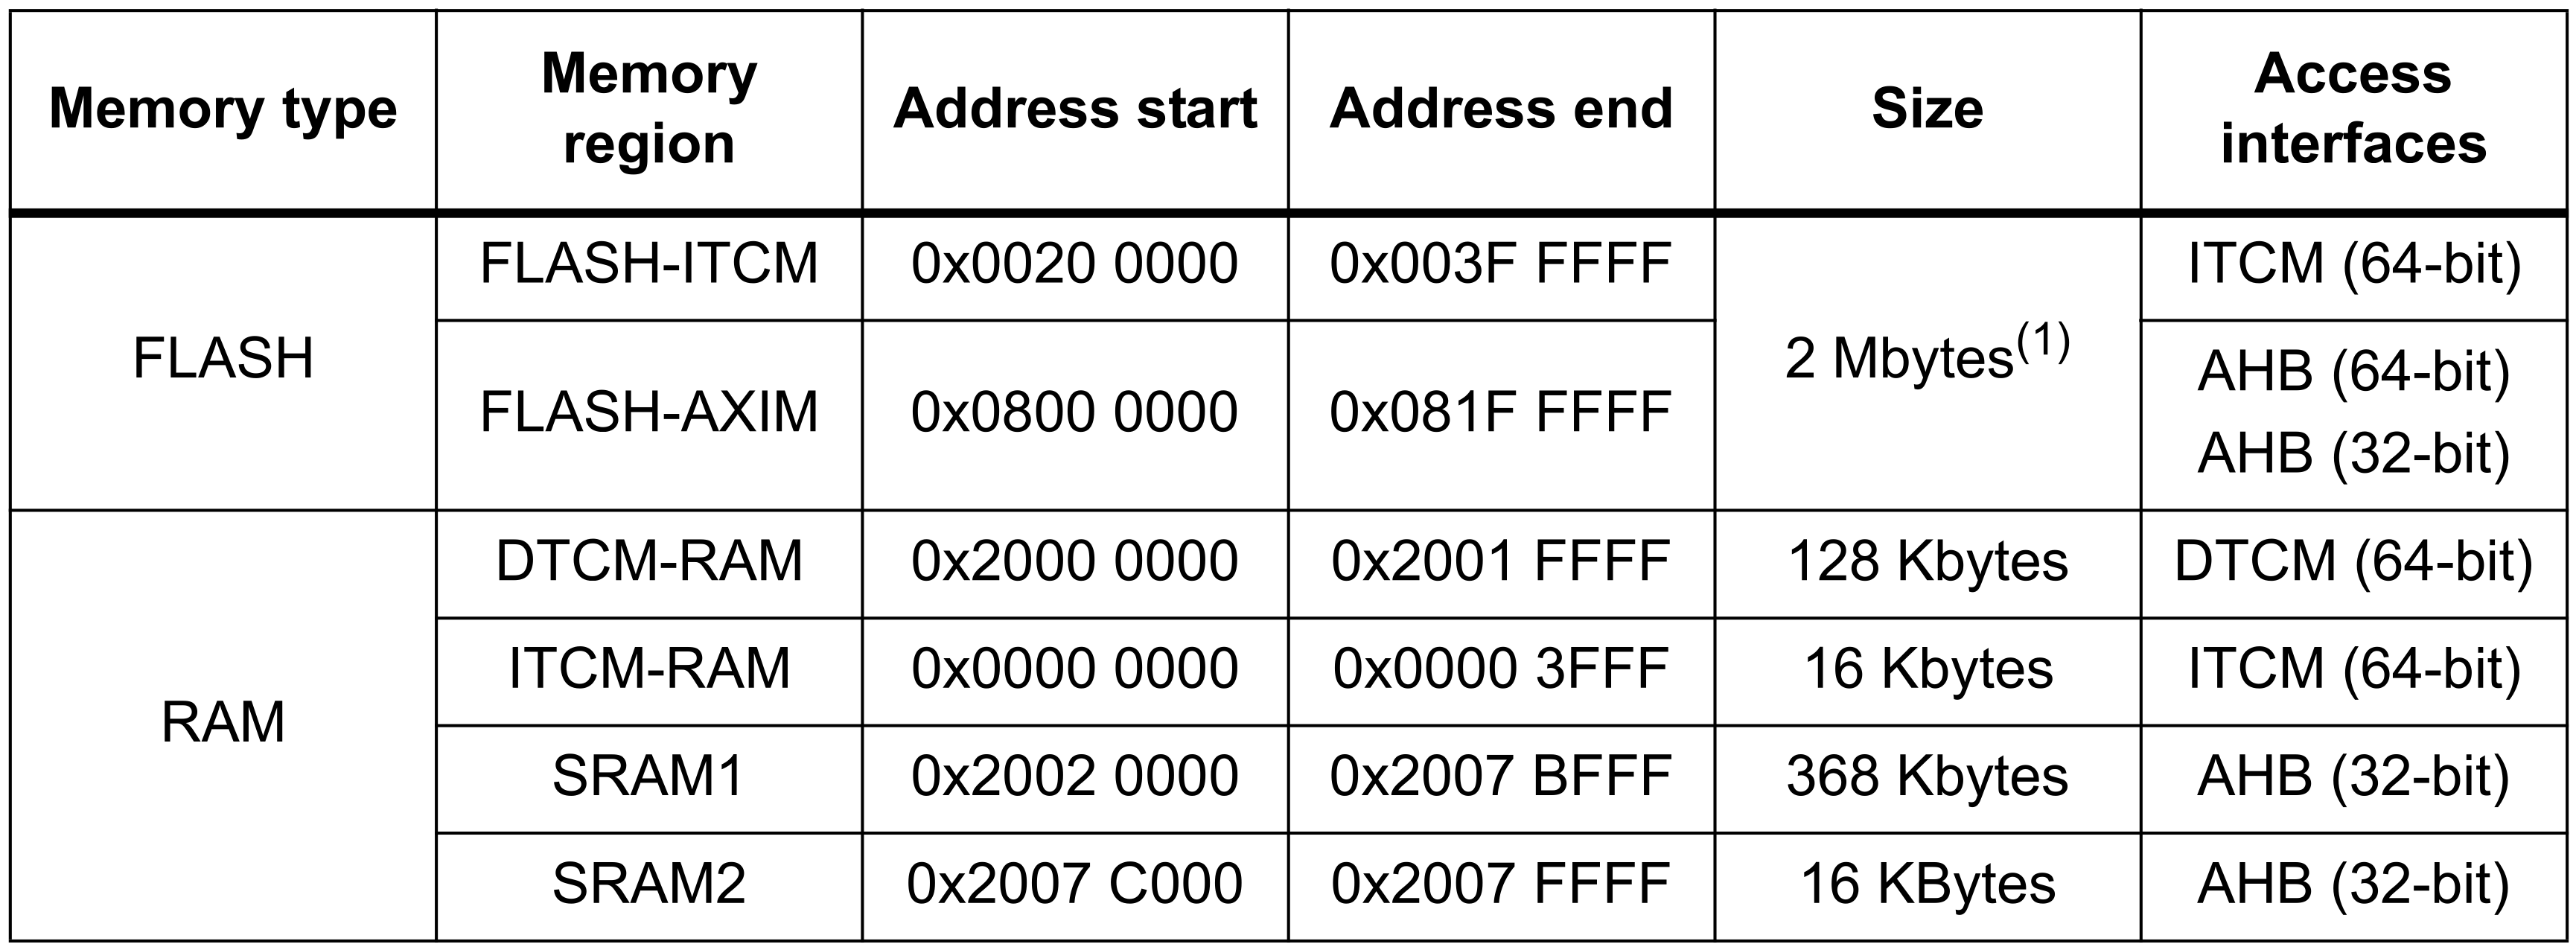
\includegraphics[width=1\textwidth]{assets/internal_mem_table}
    \caption{STM32F7 Speicheradressen \cite[S. 14]{an4667}}
    \label{fig:internal_mem_table}
\end{figure}

Aus der Abbildung \ref{fig:internal_mem_table} wird deutlich, dass der Flash ab
der Adresse $0x0800 0000$ über den AXI-Bus angesprochen wird. Diese Adresse ist
auch im Linker-Skript (\ref{code:linker_script}) standardmäßig für den Flash
festgelegt. Daher kann der Instruktionscache über den AXI-Bus für den Flash
genutzt werden, sofern der Boot-Pin sowie die assoziierten
Registerkonfigurationen (\mintinline{text}|BOOT_ADDx|) korrekt eingestellt sind
\cite[S. 28]{stm32_datasheet} und die Firmware an die Standardadresse geflasht
und gestartet wird.

\begin{code}
\begin{minted}{c}
MEMORY
{
RAM (xrw)      : ORIGIN = 0x20000000, LENGTH = 512K
FLASH (rx)      : ORIGIN = 0x8000000, LENGTH = 2048K
}
\end{minted}
    \captionof{listing}{Definition Speicherbereich im Linker-Script für STM32F7}
    \label{code:linker_script}
\end{code}

Um Caches zu nutzen, bietet die \ac{HAL} von STM32 dedizierte Funktionen
(\ref{code:hal_cache_api}) als API an \cite[S. 4]{an4839}:

\begin{code}
\begin{minted}{c}
void SCB_EnableICache(void)
void SCB_EnableDCache(void)
void SCB_DisableICache(void)
void SCB_DisableDCache(void)
void SCB_InvalidateICache(void)
void SCB_InvalidateDCache(void)
void SCB_CleanDCache(void)
void SCB_CleanInvalidateDCache(void)
\end{minted}
    \captionof{listing}{Cache-Funktionen}
    \label{code:hal_cache_api}
\end{code}

\paragraph{Cache-Leerung}

Bei einer Cache-Leerung (cache clean) werden die modifizierten Cache-Zeilen, die
vom Prozessor während der Programmausführung aktualisiert wurden, zurück in den
Hauptspeicher geschrieben. Dieser Vorgang wird gelegentlich auch als „flush”
bezeichnet.

\paragraph{Cache-Invalidierung}

Eine Cache-Invalidierung markiert hingegen den Cache als ungültig, sodass bei
dem nachfolgenden Zugriff auf die assoziierten Daten diese zwingend erneut aus
dem Hauptspeicher geladen werden und der Cache entsprechend aktualisiert wird.

\subsubsection{Cache-Kohärenz} \label{sec:cache_coherency}

Bei der Nutzung von Caches kann für Speicherbereiche, die mit dem DMA-Controller
geteilt werden, ein Cache-Kohärenzproblem (cache coherency) auftreten, da der
Prozessor in diesem Fall nicht mehr der einzige Master ist, der auf diese
Speicherbereiche zugreift.

Damit der DMA-Controller stets auf korrekte Daten zugreifen kann, ist eine
manuelle Cache-Leerung \textit{nach} jedem Schreibvorgang von Seiten der CPU
erforderlich \cite[S. 6]{an4839}. Ohne diesen Schritt würden die Änderungen
nicht umgehend im Speicher widergespiegelt werden und der DMA-Controller würde
in der Zwischenzeit auf die veralteten und somit ungültigen Daten zugreifen.

Bei Daten, die aus einem Speicherbereich gelesen werden, der auch vom
DMA-Controller modifiziert werden kann, ist \textit{vor} jedem Lesevorgang eine
Cache-Invalidierung notwendig \cite{embeddedexpert_cache}. Da der DMA-Controller
asynchron und unabhängig von der CPU schreiben kann, sind die gecachten Daten
immer potenziell veraltet und müssen stets manuell aktualisiert werden.

\subsection{Data Watchpoint and Trace Unit} \label{sec:dwt}

Für die Echtzeitfähigkeitsanalyse der Steuerungssoftware wird eine Methode
benötigt, die Code- bzw. Ausführungsabschnitte flexibel messen kann. Da es sich
dabei um eine Multithreaded-Anwendung handelt, muss gewährleistet sein, dass die
Messungen trotz präemptives Scheduling, auftretender Interrupts sowie Software-
und Hardwareoptimierungen threadsicher und präzise durchgeführt werden. Die
endgültige Lösung muss garantieren, dass dabei keine Race Conditions entstehen
und auch die Zeiterfassung selbst keinen nennenswerten Overhead verursacht.

Daher bietet sich die DWT als geeigneter Ansatz zur Protokollierung von
Laufzeiten an. Die DWT ist eine in ARM-Prozessoren eingebaute Debugging-Einheit,
die unter anderem ein funktionsreiches Profiling mittels verschiedener Zähler
unterstützt \cite{ARMv7_ref_man_dwt_profiling}. Ein für diese Arbeit zentraler
Baustein ist der Zyklenzähler \mintinline{c}|DWT_CYCCNT|, der bei jedem CPU-Takt
inkrementiert wird, solange sich der Prozessor nicht im Debug-Zustand befindet
\cite{ARMv7_ref_man_dwt_cycle}. Die DWT ermöglicht eine Laufzeit-Protokollierung
mit zyklengenauer Präzision „unter normalen Betriebsbedingungen”
\cite{ARMv7_ref_man_dwt_profiling}.

Ein Beispiel hierfür ist Segger SystemView, ein Echtzeitanalyse-Tool, das die
DWT nutzt, um Live-Code-Profiling auf eingebetteten Systemen durchzuführen
\cite{SEGGER_SystemView}. Das Tool nutzt den DWT-Zyklenzähler, indem die
Funktion \mintinline{c}|SEGGER_SYSVIEW_GET_TIMESTAMP()| für
Cortex-M3/4/7-Prozessoren einfach auf die hardkodierte Registeradresse des
Zyklenzählers~\cite{Arm_DWT_Programmers_Model} zugreift \cite[S.
65]{Segger_SystemView_manual}, anstatt die interne Funktion
\linebreak \mintinline{c}|SEGGER_SYSVIEW_X_GetTimestamp()| aufzurufen.
